% DRAFT analysis-paper v1 (2026-10-27). Every number is copied from a results file in this repo (path in a comment or
% caption). Not paper-ready: rule 11 (independent check of code, numbers and the proofs; docs/RULE11_CHECKLIST.md)
% has not been signed off.
\documentclass[11pt]{article}
\usepackage[margin=1in]{geometry}
\usepackage{amsmath,amssymb,amsthm,booktabs,natbib,hyperref,graphicx}
\newtheorem{proposition}{Proposition}
\newtheorem{theorem}{Theorem}
\newcommand{\todo}[1]{\textbf{[TODO: #1]}}
\title{When Does Head Selection Matter? Output-Space Redundancy, Closed-Form Compensation, and Global Allocation in Retraining-Free Transformer Pruning}
\author{Anonymous}
\date{}
\begin{document}
\maketitle

\begin{abstract}
Retraining-free pruning of fine-tuned encoders removes attention heads and feed-forward neurons using a small
calibration set and repairs the damage with a closed-form least-squares (LS) update. Which units to remove (selection) and how to
repair the rest (compensation) are usually evaluated together. We separate them in a sequence of pre-registered
experiments on BERT-base, and most of our hypotheses are not supported. (i) Attention-pattern similarity, the natural
redundancy signal for heads, is blind to how a head mixes values; on four of five GLUE tasks most head pairs that it
calls near-identical have dissimilar outputs. (ii) At 50\% of heads per layer, once the kept heads are refit by LS,
five selectors are statistically indistinguishable; compensation, not selection, carries the recovery. (iii) A global,
refit-aware allocation over heads and neurons (GRP) lowers the logit KL to the teacher well below official K-prune on
SST-2 but not on MRPC, so its pre-registered calibration gate fails and no accuracy comparison was run. (iv) K-prune's
advantage over a module-output refit is fully explained by a drift-corrected least-squares target; with that
compensation held equal, which selection rule wins depends on the task. We make no claim of improved accuracy or speed
over the state of the art, and no latency was measured.
\end{abstract}

\section{Introduction}
Retraining-free (post-training) structured pruning removes attention heads and feed-forward (FFN) neurons from a
fine-tuned transformer using only a small calibration set, and repairs the damage with a closed-form or few-second
weight update instead of fine-tuning~\citep{kwon2022fast,park2024kprune,nova2023kcm}. Two questions are usually
entangled in this setting: \emph{which} units to remove (selection), and \emph{how} to compensate for the removed units
(reconstruction). This paper separates them with pre-registered experiments.

Our starting point was a representation of each head by its normalized attention pattern and a fidelity-based coverage
objective for choosing redundant heads. We show that attention-pattern similarity is a poor redundancy signal: it is
blind to how a head mixes values (Proposition~\ref{prop:blind}), and on BERT-base, on four of five GLUE tasks, most
head pairs that it calls near-identical produce dissimilar outputs (Section~\ref{sec:diag}). Moving the similarity to the head's output operator
gives a coverage bound on the merge error that ranks subsets well (Theorem~\ref{thm:bound}), yet in a pre-registered
factorial over five GLUE tasks and five calibration seeds, once the remaining heads are refit by least squares the
choice of selector barely matters at 50\% of heads per layer (Section~\ref{sec:v14}). We then asked whether a global,
refit-aware allocation over heads and FFN neurons (GRP) improves on the two official retraining-free baselines
(Section~\ref{sec:v15}). It does so on SST-2 but not on MRPC, and a transplant analysis shows that K-prune's own
advantage over a module-output refit is a drift-corrected least-squares target (Section~\ref{sec:v16}); after
equalizing compensation the remaining effect of selection is task-dependent. All of this is negative or descriptive
evidence, and the paper is framed accordingly.

\paragraph{Contributions.} (i) A characterization of when attention-pattern similarity fails as a redundancy proxy, with
a proposition and a measurement on BERT-base. (ii) An output-space coverage bound for merging pruned heads into kept
heads, with its tightness measured. (iii) A pre-registered selector $\times$ compensation factorial showing that, at
moderate sparsity, closed-form compensation explains most of the retraining-free recovery and selectors are
statistically indistinguishable after it. (iv) A pre-registered calibration gate for a global refit-aware allocation (GRP) against reproduced official Kwon et
al.\ and K-prune code, with the task-dependent outcome; (v) a decomposition showing that K-prune's compensation is
exactly a drift-corrected LS refit, and a selection $\times$ compensation table that holds compensation fixed.
Hypotheses, thresholds and analysis code were fixed before the corresponding data were seen, with one exception stated
in Section~\ref{sec:prereg}; negative results are reported as such.

\section{Related work}
\paragraph{Head and structured pruning.} Many heads can be removed with little loss~\citep{michel2019sixteen,voita2019analyzing};
head pruning has also been cast as differentiable subset selection~\citep{li2021dsp}. Training-based structured pruning
recovers accuracy by fine-tuning~\citep{sanh2020movement,xia2022cofi}.
\paragraph{Retraining-free pruning of encoders.} \citet{kwon2022fast} search Fisher-based masks over heads and FFN
filters under a FLOPs constraint and rescale the kept units by layer-wise least squares. KCM prunes with unlabeled data and
no gradients~\citep{nova2023kcm}. K-prune scores units by predictive and representational knowledge per FLOP and tunes the
weights of each pruned sublayer by least squares~\citep{park2024kprune}. LIAR~\citep{wang2024liar} reconstructs pruned outputs by linear interpolation over the preserved weights, and
Global-Pruner~\citep{yao2024globalpruner} searches masks globally with reinforcement learning before a mask-tuning step.
OSSCAR solves a layer-wise combinatorial
reconstruction problem with local search~\citep{meng2024osscar}; CORP folds closed-form ridge compensation into the
weights~\citep{zhang2026corp}; Neuron Merging folds removed neurons into kept ones~\citep{kim2020neuron}. Olica applies closed-form linear
calibration after structured pruning of large language models~\citep{he2025olica}.
\paragraph{Allocation and repairability.} The idea that sparsity should be allocated by how much damage later layers
absorb or a repair removes is recent: \citet{jing2026absorption} correct layer-wise rates by an inter-layer
perturbation-absorption ratio (decoder LLMs, unstructured), and \citet{zhan2026repairability} use the fraction of
damage left after a channelwise repair as an allocation diagnostic (CNNs). Our setting is structured pruning of encoders
with an exact refit.
\paragraph{One-shot pruning of large models.} SparseGPT, Wanda, LLM-Pruner, SliceGPT and ZipLM prune large decoders with
little or no retraining~\citep{frantar2023sparsegpt,sun2024wanda,ma2023llmpruner,ashkboos2024slicegpt,kurtic2023ziplm}.
\paragraph{Positioning.} Removal costs from least-squares downdates and closed-form compensation are each known. Our
claims are (a) an analysis of which redundancy notion matters, (b) controlled, pre-registered evidence on the relative
roles of selection and compensation, and (c) a negative result for a global refit-aware allocation, together with the identification of K-prune's
compensation mechanism. None of these is a new pruning principle.

\section{Setup and notation}
For one layer, let $Z_h\in\mathbb{R}^{N\times d}$ be the context vectors of head $h$ over the $N$ non-padding calibration
tokens ($d=64$, $H=12$ heads), $Z=[Z_1,\dots,Z_H]$, and $W_O=[W_1;\dots;W_H]$ the attention output projection with
$W_h\in\mathbb{R}^{d\times D}$. The attention output is $Y=ZW_O=\sum_h Z_hW_h$. Everything below depends on the data only
through the Gram matrix $G=Z^\top Z$. Keeping a set $S$ of heads, the least-squares (LS) compensation is
$\widehat W_S=\arg\min_{V}\|Y-Z_SV\|_F^2$ (with a small ridge in practice).

\paragraph{Output fidelity.} For heads $i,j$ define
$F_{ij}=\big(\|Z_i^\top Z_j\|_*/(\|Z_i\|_F\|Z_j\|_F)\big)^2\in[0,1]$, the squared Uhlmann fidelity between the head
operators. The attention-pattern alternative represents head $h$ by $\rho_h=A_hA_h^\top/\mathrm{tr}(A_hA_h^\top)$ for
its attention matrix $A_h$.

\section{Theory}
\begin{proposition}[Attention-pattern fidelity is blind to value mixing]\label{prop:blind}
If $A_j=A_iQ$ with $QQ^\top=I$ (for example, a permutation of keys), then $\rho_j=\rho_i$, so the attention-pattern
fidelity of heads $i$ and $j$ is 1, while their outputs $A_iV_i$ and $A_jV_j=A_iQV_j$ can be arbitrary.
\end{proposition}
\begin{proof}
$(A_iQ)(A_iQ)^\top=A_iQQ^\top A_i^\top=A_iA_i^\top$. The outputs depend on $QV_j$, which $\rho$ does not constrain.
\end{proof}

\begin{proposition}[Scaled-orthogonal Procrustes residual]\label{prop:proc}
$\min_{s\in\mathbb{R},\,U^\top U=I}\|Z_j-sZ_iU\|_F=\|Z_j\|_F\sqrt{1-F_{ij}}$.
\end{proposition}
\begin{proof}
For fixed $U$ the optimal $s=\mathrm{tr}(U^\top Z_i^\top Z_j)/\|Z_i\|_F^2$ and the squared residual is
$\|Z_j\|_F^2-\mathrm{tr}(U^\top Z_i^\top Z_j)^2/\|Z_i\|_F^2$. Over orthogonal $U$ the trace is maximized by the polar
factor of $Z_i^\top Z_j$, where it equals $\|Z_i^\top Z_j\|_*$ (von Neumann's trace inequality).
\end{proof}

\begin{theorem}[Output-space coverage bound]\label{thm:bound}
Let $S$ be the kept heads and assign each pruned head $j$ to $\pi(j)=\arg\min_{i\in S}\sqrt{1-F_{ji}}$. Merging
$W_{\pi(j)}\leftarrow W_{\pi(j)}+R_jW_j$ with the Procrustes map $R_j$ of Proposition~\ref{prop:proc} gives
\[\|Y-\widehat Y_{\mathrm{merge}}\|_F\le B(S)=\sum_{j\notin S}w_j\min_{i\in S}\sqrt{1-F_{ji}},\qquad
w_j=\|W_j\|_2\,\|Z_j\|_F,\]
and the (unregularized) LS-refit error is at most the merge error.
\end{theorem}
\begin{proof}
$Y-\widehat Y_{\mathrm{merge}}=\sum_{j\notin S}(Z_j-Z_{\pi(j)}R_j)W_j$; apply the triangle inequality,
$\|MW_j\|_F\le\|M\|_F\|W_j\|_2$ and Proposition~\ref{prop:proc}. The merged weights are feasible for the LS problem
over $Z_S$, so the LS optimum is no larger.
\end{proof}
Since $B(S)=\sum_{j\notin S}w_j-f(S)$ with $f$ a weighted facility-location function, greedy maximization of $f$ carries
the usual $(1-1/e)$ guarantee on $f$; this is an additive statement, not a guarantee on $B$ or on accuracy.

\section{Methods compared}
\paragraph{V14 factorial (heads only, $k=6$ of 12 per layer).} Selectors: output-space coverage (BCM, greedy on $f$),
Fisher top-$k$ (Michel gate sensitivity), magnitude top-$k$ ($w_j$), greedy exact LS, and attention-pattern coverage.
Compensation: none, merge (Theorem~\ref{thm:bound}), one-shot LS, sequential LS (layer by layer, teacher targets,
student inputs).
\paragraph{V15: global reconstruction pruning (GRP).} Units are heads (blocks of $d$ features of $Z$) and FFN neurons
(single features of the GELU activation entering $W_2$), in all layers. For a module with augmented Gram $G$ (a constant
feature fits the bias) and refit $V=P\,G_{S:}W$, $P=(G_{SS}+\lambda I)^{-1}$, removing unit $R$ increases the refit
objective by $\Delta E_R=\mathrm{tr}(V_R^\top P_{RR}^{-1}V_R)$ (exact block downdate). GRP repeatedly removes the units
with the smallest $s_m\Delta E_R/\mathrm{MAC}_R$ across all modules, where $s_m$ is the expected Fisher of the module
output under teacher-sampled labels, until the MAC budget of \citet{kwon2022fast} is met; it then prunes the matrices
physically and refits $W_O$ and $W_2$ (with biases) layer by layer. K-prune~\citep{park2024kprune} is the closest prior
method; GRP differs in the refit-aware cost (error \emph{after} the optimal refit rather than the output norm), the
module-output sensitivity, and a single global greedy instead of a per-sublayer threshold.

\section{Pre-registered protocol}\label{sec:prereg}
Models: fine-tuned BERT-base~\citep{devlin2019bert} checkpoints with pinned revisions; tasks from
GLUE~\citep{wang2018glue} (SST-2, MRPC development; RTE, QNLI, CoLA confirmatory for V14) and, for V15,
SQuAD~v1.1~\citep{rajpurkar2016squad}. Calibration: train only (512 examples for V14, 2048 for V15), five seeds
(7, 42, 77, 123, 2024); evaluation on the full validation split. Statistics: paired cluster bootstrap over
(seed $\times$ example), 10{,}000 resamples, Holm across confirmatory tasks; Random is a distribution of 100 masks.
Decision rules and thresholds were committed before any data (repository file \texttt{docs/PROJECT\_STATE.md}).
\paragraph{Disclosure.} The V17 hypothesis (drift-corrected compensation for GRP) was registered after the V15 and V16
development data on MRPC and SST-2 had been seen, under the author's standing autonomy grant and without a separate
confirmation step. MRPC and SST-2 are therefore development tasks for GRP, and V17 is not an independent confirmation.
No confirmatory data (QNLI, MNLI-m, QQP validation splits) were used for any GRP or GRP-R result. The gate metric in
V15--V17 is the logit KL to the teacher on 512 held-out \emph{training} rows, not validation accuracy.

\section{Results}
\subsection{Attention similarity versus output similarity}\label{sec:diag}
% results/v14_bcm_diag/4bd649f (CPU diagnostic, seed 7, calibration data only)
On SST-2 and MRPC (seed 7), 54 and 36 of the 792 within-layer head pairs have attention-pattern fidelity above 0.99;
of these, 39 and 35 have output fidelity below 0.5. The median per-layer Spearman correlation between the two
similarities is 0.437 and 0.263. The coverage bound ranks random subsets almost as the true merge error does (median
per-layer Spearman 0.929 and 0.959) but is loose (median ratio 3.26 and 3.12). At layer level, BCM (relative LS error
0.334 / 0.304) is close to the exhaustive optimum (0.320 / 0.296) and to greedy exact LS (0.321 / 0.297), better than
Fisher (0.359 / 0.402) and attention coverage (0.417 / 0.391), but tied by magnitude top-$k$ (0.334 / 0.307).
Figure~\ref{fig:pairs} shows every head pair: the pairs that attention-pattern similarity calls near-identical are
spread over output fidelities from about 0.1 to 0.5.
\begin{figure}[t]\centering
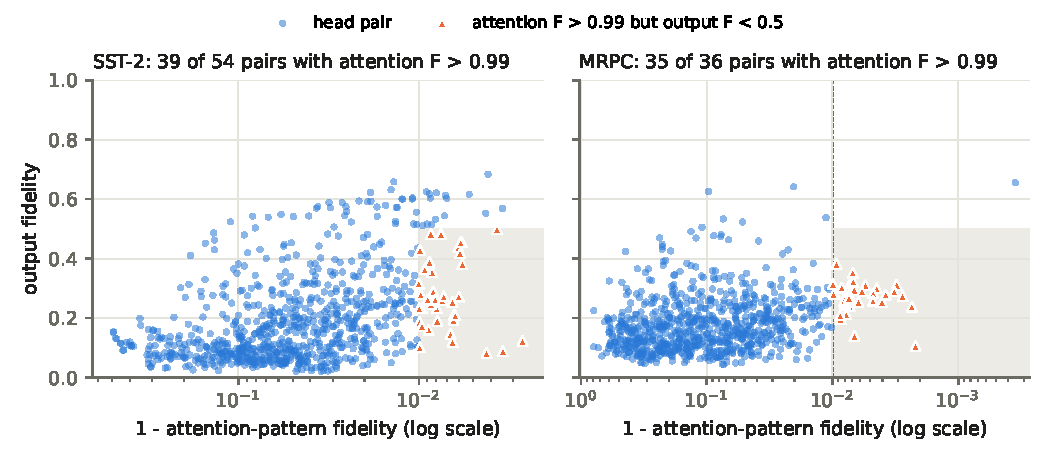
\includegraphics[width=\linewidth]{figs/fig_pairs.pdf}
\caption{Attention-pattern fidelity versus output fidelity for all 792 within-layer head pairs of BERT-base
(calibration data, seed 7). Shaded: attention fidelity above 0.99 but output fidelity below 0.5. Source:
\texttt{results/v14\_pairs/71cb52d}.}\label{fig:pairs}
\end{figure}
Over all five tasks and five calibration seeds (\texttt{results/v14\_bcm\_diag/full\_be03d75/diag\_summary.json}),
the share of attention-near-identical pairs (fidelity above 0.99) whose output fidelity is below 0.5 is 72\% on
SST-2 (195 of 270), 97\% on MRPC (179/184), 92\% on RTE (57/62) and 82\% on QNLI (23/28), but only 20\% on CoLA
(38/189), whose inputs are short single sentences; the blindness is therefore real but task-dependent. The
other diagnostics replicate on every task: the coverage bound ranks random subsets like the true merge error
(median per-layer Spearman 0.915--0.955) while overestimating it about threefold (median ratio 3.12--3.26);
greedy exact LS is within 0.001--0.002 of the exhaustive per-layer optimum in mean relative error; BCM is within
0.008--0.022 of the optimum, below Fisher top-$k$ and attention coverage on every task, and level with magnitude
top-$k$ (difference at most 0.006, in both directions).

\subsection{Selection versus compensation (V14, pre-registered)}\label{sec:v14}
% results/v14_bcm/9c4b999 ; v14_verdicts.json
\begin{table}[t]\centering\small
\caption{Validation metric (accuracy; CoLA: MCC), mean over 5 calibration seeds, BERT-base, 6 of 12 heads kept in every
layer. Random: mean $\pm$ sd over 100 masks. Source: \texttt{results/v14\_bcm/9c4b999}.}
\begin{tabular}{lccccc}\toprule
 & SST-2 & MRPC & RTE & QNLI & CoLA\\\midrule
Unpruned & 0.9243 & 0.8775 & 0.7256 & 0.9154 & 0.5339\\
Random (no comp.) & 0.879$\pm$0.018 & 0.730$\pm$0.064 & 0.589$\pm$0.040 & 0.700$\pm$0.092 & 0.228$\pm$0.143\\
Attention coverage, none & 0.8784 & 0.7328 & 0.5884 & 0.5669 & 0.0093\\
Attention coverage, seq.\ LS & 0.9050 & 0.7814 & 0.6787 & 0.8289 & 0.5141\\
BCM, none & 0.9142 & 0.8186 & 0.6368 & 0.8559 & 0.4970\\
BCM, merge & 0.9174 & 0.8667 & 0.6477 & 0.8816 & 0.5452\\
BCM, seq.\ LS & 0.9193 & 0.8564 & 0.7083 & 0.8962 & 0.5429\\
Fisher, seq.\ LS & 0.9151 & 0.8583 & 0.6953 & 0.8992 & 0.5402\\
Magnitude, seq.\ LS & 0.9167 & 0.8598 & 0.7011 & 0.8937 & 0.5285\\
Greedy exact LS, seq.\ LS & 0.9170 & 0.8623 & 0.6960 & 0.8936 & 0.5374\\\bottomrule
\end{tabular}\end{table}
\begin{figure}[t]\centering
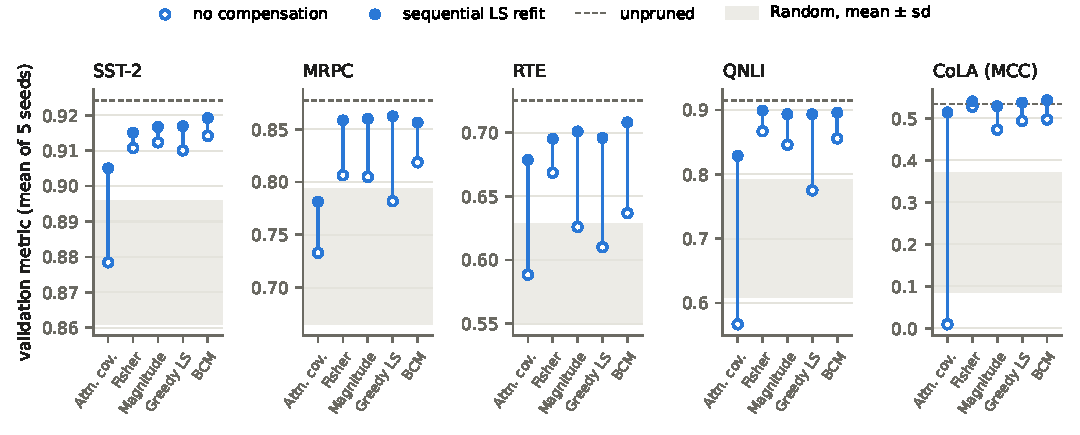
\includegraphics[width=\linewidth]{figs/fig_v14.pdf}
\caption{Selection versus compensation (V14, BERT-base, 6 of 12 heads per layer). Open circles: no compensation;
filled: sequential LS refit; mean of 5 calibration seeds. The vertical gain from compensation is larger than the
spread between selectors after compensation. Source: \texttt{results/v14\_bcm/9c4b999}.}\label{fig:v14}
\end{figure}
Sequential LS compensation raises every selector's mean on every task (Figure~\ref{fig:v14}); for BCM the paired gain is +4.03 points on QNLI
(95\% CI [+3.27, +4.82]) and +7.15 on RTE ([+2.45, +11.84]). After compensation, the pre-registered comparisons are
null: BCM minus Fisher ranges from $-0.30$ (QNLI, CI [$-0.93$, +0.36]) to +1.30 (RTE, [$-1.73$, +4.33]) points with no
Holm-significant difference on any task (H9b), and BCM versus greedy exact LS is likewise null (H9c). Merging into the
coverage-assigned head beats merging into a random kept head only on QNLI (+1.11, [+0.78, +1.45]; H9d not supported).
Attention-pattern coverage without compensation is at the Random mean on SST-2, MRPC and RTE and below it on QNLI and
CoLA. A calibration-side check confirms that the refit lowers the per-layer output error and the logit KL in every
layer, seed, selector and task examined, on held-out training data too (\texttt{results/v14\_h9a\_check/fdd808d}); the
pre-registered H9a failure for BCM and Fisher on SST-2 and MRPC reflects ceiling and sample size, not an
implementation error.

\subsection{Global allocation over heads and neurons (V15, pre-registered)}\label{sec:v15}
% Phase 1: docs/PROJECT_STATE.md (Kaggle Versions 2-4); H10: results/v15_h10/c43dd3e/h10/v15_h10_verdict.json
\paragraph{Reproduction gate.} Both official codes reproduce. K-prune on its own BERT-base checkpoints at 80\% MAC
reduction gives 84.85 on MRPC (published 84.80) and 74.20 SQuAD~v1.1 F1 (published 74.16), means over five seeds.
Kwon et al.'s checkpoints are no longer available, so their code was run on K-prune's checkpoints and the accuracy
\emph{drop} was compared with theirs (Appendix~\ref{app:repro}). The pre-registered rule passes (the drop is missed by
more than one point at most budgets only on MRPC, where the validation set has 408 examples).

\paragraph{Calibration gate (H10).} Before any accuracy run, GRP had to lower the logit KL to the teacher on 512
held-out training rows by at least 10\% relative to \emph{both} baselines at the same budget, at two or more of four
budgets, on both development tasks. Table~\ref{tab:h10} shows that it does so at every budget on SST-2, with KL 40--75\%
below K-prune, but at no budget on MRPC, where K-prune is lower at 50\% and 40\% of MACs. H10 is therefore not
supported, and following the pre-registration no accuracy comparison (H11) was run: GRP is not claimed to improve on
K-prune. The task dependence motivates the diagnosis in Section~\ref{sec:v16}.
\begin{figure}[t]\centering
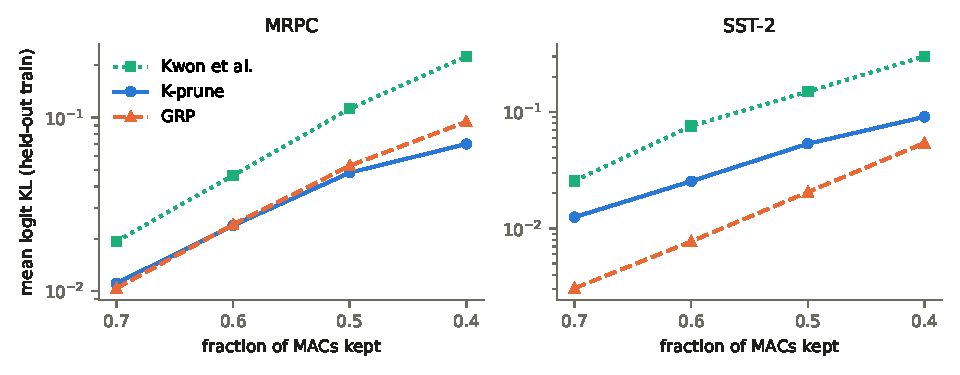
\includegraphics[width=\linewidth]{figs/fig_h10.pdf}
\caption{H10 gate: mean logit KL to the teacher (log scale) versus the fraction of MACs kept, five seeds.
Source: \texttt{results/v15\_h10/c43dd3e/h10/v15\_h10\_verdict.json}.}\label{fig:h10}
\end{figure}
\begin{table}[t]\centering\small
\caption{Mean logit KL(teacher $\|$ pruned) on 512 held-out training rows, five calibration seeds, BERT-base, by
fraction of MACs kept. Kwon et al.\ and K-prune: official code on the same checkpoints and calibration rows. Source:
\texttt{results/v15\_h10/c43dd3e}.}\label{tab:h10}
\begin{tabular}{llcccc}\toprule
Task & Method & 0.7 & 0.6 & 0.5 & 0.4\\\midrule
MRPC & Kwon et al. & 0.0194 & 0.0464 & 0.1123 & 0.2249\\
 & K-prune & 0.0111 & 0.0239 & 0.0481 & 0.0703\\
 & GRP & 0.0104 & 0.0242 & 0.0527 & 0.0946\\\midrule
SST-2 & Kwon et al. & 0.0256 & 0.0758 & 0.1497 & 0.3009\\
 & K-prune & 0.0125 & 0.0254 & 0.0534 & 0.0909\\
 & GRP & 0.0031 & 0.0077 & 0.0205 & 0.0543\\\bottomrule
\end{tabular}\end{table}

\subsection{Why the advantage is task-dependent (V16, pre-registered diagnosis)}\label{sec:v16}
% results/v16_stageA/b2b444e ; v16_stageA_verdict.json
A second pre-registered study decomposed the gap on the development tasks by transplanting parts between the two
methods (same calibration and held-out rows). Applying GRP's refit to K-prune's own selected units makes the KL 34--60\%
\emph{worse} than K-prune's own compensation. Restricting GRP to K-prune's per-module unit counts while letting it choose
units inside each module does not help on either task. Removing GRP's sensitivity weight lowers the KL on MRPC at 50\%
of MACs (0.0445 vs 0.0527) but costs most of the SST-2 advantage (0.0480 vs 0.0205). A probe of the exchange rate
between local refit error and logit KL was too noisy at a 2\% removal to support a correction. No transplant met the
pre-registered criterion, so the study stopped before any confirmatory run (branch A-3). Reading K-prune's code shows one
concrete difference in compensation: its least-squares target is the teacher's sublayer output minus the
\emph{student's} residual input, which also cancels drift accumulated in earlier layers, whereas GRP fits the
module output alone.

% results/v17_rdev/195c18f ; v17_rdev_verdict.json
A third pre-registered study tested that difference directly. Refitting K-prune's selected units with the
drift-corrected target reproduces K-prune's own KL within 3\% on both tasks and both budgets, so this target accounts
fully for K-prune's compensation advantage. Giving GRP the same compensation (GRP-R) does not remove its MRPC deficit:
its KL is 1.19 and 1.29 times K-prune's at 50\% and 40\% of MACs, against 0.31 and 0.50 on SST-2. The pre-registered gate
failed, and no confirmatory run was made. Table~\ref{tab:factorial} holds compensation fixed: the remaining
difference is selection, and which selection rule wins depends on the task (Figure~\ref{fig:factorial}).
\begin{table}[t]\centering\small
\caption{Selection $\times$ compensation on held-out training rows: mean KL as a ratio to official K-prune at the same
budget (five seeds; lower is better). Sources: \texttt{results/v16\_stageA/b2b444e}, \texttt{results/v17\_rdev/195c18f},
\texttt{results/v15\_h10/c43dd3e}.}\label{tab:factorial}
\begin{tabular}{llcccc}\toprule
Selection & Compensation & MRPC 0.5 & MRPC 0.4 & SST-2 0.5 & SST-2 0.4\\\midrule
K-prune & module-output LS & 1.48 & 1.53 & 1.34 & 1.60\\
K-prune & drift-corrected LS & 0.98 & 0.97 & 1.00 & 1.00\\
GRP & module-output LS & 1.10 & 1.35 & 0.38 & 0.60\\
GRP & drift-corrected LS & 1.19 & 1.29 & 0.31 & 0.50\\\bottomrule
\end{tabular}\end{table}
\begin{figure}[t]\centering
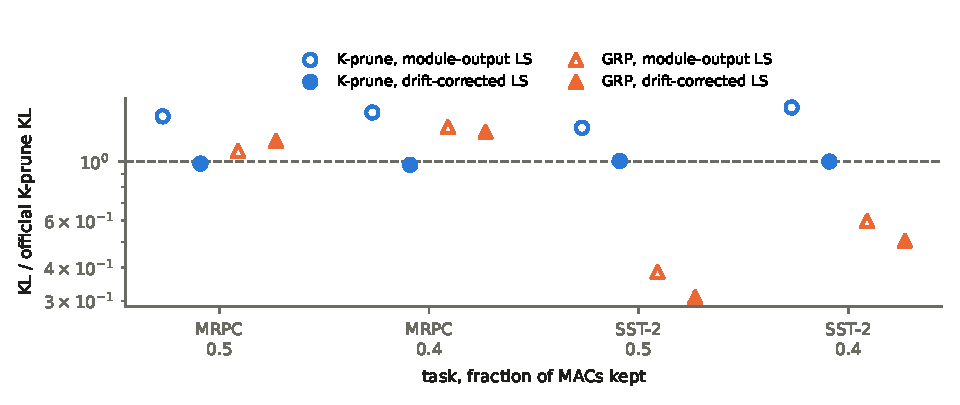
\includegraphics[width=\linewidth]{figs/fig_factorial.pdf}
\caption{Table~\ref{tab:factorial} as a plot (log scale; the dashed line is official K-prune). Open markers: module-output
refit; filled: drift-corrected refit. Source: \texttt{results/v16\_stageA/b2b444e}, \texttt{results/v17\_rdev/195c18f},
\texttt{results/v15\_h10/c43dd3e}.}\label{fig:factorial}
\end{figure}

\section{Limitations}
\begin{itemize}\setlength\itemsep{0pt}
\item One model family (BERT-base) and two development tasks for GRP; no RoBERTa, no decoder, no larger model.
\item The V15--V17 gate metric is the logit KL on held-out training rows. It is a calibration-side quantity; we
did not run the accuracy comparison (H11), so no accuracy conclusion about GRP or GRP-R is drawn.
\item No latency or speed was measured. V14 results are functional masks; V15--V17 refit physically pruned matrices, but
no wall-clock or FLOP claims are made.
\item MRPC has 408 validation examples, so accuracy differences of one to two points are within noise there.
\item V14 uses a single, uniform sparsity level (6 of 12 heads); its Kaggle run did not record exact package version
strings. The V17 hypothesis was registered after the V15/V16 development data were seen (Section~\ref{sec:prereg}).
\item The three proofs have not yet been checked by an independent reader (\texttt{docs/RULE11\_CHECKLIST.md}).
\end{itemize}

\appendix
\section{Reproducibility details for the baselines (V15)}\label{app:repro}
\paragraph{Official code.} Kwon et al.: \texttt{github.com/WoosukKwon/retraining-free-pruning} at commit 806ac5a6;
K-prune: \texttt{github.com/snudm-starlab/K-prune} at commit 9ca629a1. Each runs in its own environment (Python 3.9,
PyTorch 1.13.1, Transformers 4.12.0, CuPy; and Python 3.10, PyTorch 1.12.1, Transformers 4.25.1). Exactly four lines
of each \texttt{main.py} are changed: the calibration sampling line reads a fixed list of training-row indices
(identical for all methods), and two calls save teacher and pruned-model outputs on held-out training rows and on the
validation split; without the index file the code path equals the original. The diffs are released with the code.
\paragraph{Budgets.} Both codes count MACs with the same per-head and per-neuron formulas (K-prune reports FLOPs =
2 MACs) at the task's average development-set sequence length (170 for SQuAD); GRP uses the same function. Kwon's
\texttt{--constraint} is the fraction of MACs kept and K-prune's the fraction removed, so a budget $c$ is passed as
$c$ and $1-c$ respectively.
\paragraph{Checkpoints.} Kwon et al.'s released checkpoints are no longer downloadable; following a dated amendment
made before any baseline run, Kwon's code is reproduced on K-prune's released BERT-base checkpoints by comparing the
accuracy drop relative to the unpruned model with the drop reported by Kwon et al. All comparative runs use the
pinned public checkpoints (revisions in the released code); the MNLI checkpoint's classifier rows are permuted once to the GLUE
label order (mapping fixed from training data).
\paragraph{Phase~1 numbers.} K-prune, \texttt{--constraint 0.8}, seeds 0--4: MRPC accuracy 0.8431, 0.8431, 0.8505,
0.8603, 0.8456 (mean 0.8485; published 84.80); SQuAD~v1.1 F1 74.73, 73.41, 73.71, 74.34, 74.81 (mean 74.20; published
74.16). Kwon et al.'s code on K-prune's checkpoints, seeds 0--4, mean accuracy at 70/60/50\% of MACs: MRPC 0.8814 /
0.8495 / 0.8245, SST-2 0.9190 / 0.9126 / 0.8991; unpruned under the same evaluation code: MRPC 0.8701, SST-2 0.9312.
Drops versus Kwon et al.'s reported drops: MRPC $+1.13$ vs $-0.2$, $-2.06$ vs $-1.0$, $-4.56$ vs $-3.1$; SST-2 $-1.22$ vs
$-0.6$, $-1.86$ vs $-1.1$, $-3.21$ vs $-2.0$. The pre-registered stop rule (miss by more than one point at most budgets
on \emph{both} tasks) does not fire: MRPC misses at three budgets, SST-2 at one.

\bibliographystyle{plainnat}
\bibliography{refs}
\end{document}
